\documentclass[10pt,twocolumn,letterpaper]{article}

\usepackage{cvpr}
\usepackage{times}
\usepackage{epsfig}
\usepackage{graphicx}
\usepackage{amsmath}
\usepackage{amssymb}
\usepackage{hyperref}


% Include other packages here, before hyperref.

% If you comment hyperref and then uncomment it, you should delete
% egpaper.aux before re-running latex.  (Or just hit 'q' on the first latex
% run, let it finish, and you should be clear).
\usepackage[pagebackref=true,breaklinks=true,letterpaper=true,colorlinks,bookmarks=false]{hyperref}
\cvprfinalcopy



% Pages are numbered in submission mode, and unnumbered in camera-ready
\ifcvprfinal\pagestyle{empty}\fi
\begin{document}

%%%%%%%%% TITLE
\title{Lockdown Monitoring}
\author{Aryan Dubey\\
International Institute Of Information Technology Hyderabad\\
{\tt\small aryan.dubey@research.iiit.ac.in}
}

\maketitle
%\thispagestyle{empty}

%%%%%%%%% ABSTRACT
\begin{abstract}
   As cases of COVID-19 is increasing in our campus, a lot of people are getting infected because they are not following the prevention measures, monitoring in this case is very important and it can be done easily using software that give alert on conditions wherever someone is not following the covid measures and instruct them the right way. This paper will propose a software solution which will help in handling these situations and help in reducing the number of increasing cases in the institute.  
\end{abstract}

%%%%%%%%% BODY TEXT
\section{Introduction}
%-------------------------------------------------------------------------
\subsection{Main Problem}

As we know cases in our campus is increasing a lot. We need to take proper measures to prevent us from this situation and for this monitoring is very important. We need to track groups and restrict the movement of residents inside the campus for this. We also need to mark groups as safe or not based on the fact that they are wearing mask or not.

\subsubsection{Cluster number counting and density}
As the number of cases are increasing, we need to keep track of groups movement in the group, we have to make sure that the total number of people in a group can't cross 5, if it crosses 5 then we must be sure that no other person can enter that group or if he will enter we will give an alert to him as well as academy that the following group in an area crosses 5 students. Also, a group can be considered as safe or unsafe based on the fact that if anyone in the group is wearing or not wearing a mask. Also if members of a group are together for a long time, then we need to consider that group as an unsafe group.

%-------------------------------------------------------------------------
\subsubsection{Mask Detection}
If groups are moving inside the campus, we must need to keep track of all the people who are not wearing masks, and give alert to them and consider their group as unsafe group by an alert. Also, if any individual is moving in the campus without mask, it should also detect him.


\subsection{Result}
As the number of cases are increasing and also the situation around us is also not safe because of the pandemic. So, after implementing solution for above problems, we will get a situation where people will wear a mask every time to prevent themselves whenever they go out and if they don't do it they will get an alert and also administration and other people will also get notified on the map that there is person without mask, so they can maintain a distance from him and also if he/she will not mask the administration will contact him and tell him to wear mask. Similarly group tracing will help in managing the number of peoples in the group if they are more than then they will get an alert and also all other members around them as well as administration will also be notified to maintain distance from that group because it is a large group and try to not repeat this further. Similarly if unnecessary movements in the campus are restricted then anyone or any group going anywhere in the campus unnecessarily , they will get an alert and also administration will be notified that a group or a person are going somewhere unnecessarily in the campus and it can affect their health also at that it will check their mask and also notify administration that they are wearing masks or not. By applying these things our college will be protected and it will reduce the increasing number of cases in the campus.



%------------------------------------------------------------------------
\section{Literature Review}

Since COVID-19 is rising a lot these days and at many places we see how they are monitoring this to reduce the increasing number of cases. Here in my software i will use the following to implement my software solution to reduce this in my campus.
%-------------------------------------------------------------------------
\subsection{MRCNet for crowd detection}
Crowd detecction will play a very important role for our software-system. We can also say that it is one of important feature of our software system. Some current research works in this field 
is a novel crowd dataset, the DLR Aerial Crowd Dataset (DLR-ACD), which is composed of 33 large aerial images acquired from 16 flight campaigns over mass events with 226,291 persons annotated. To
tackle the problem of accurate crowd counting and density map estimation in aerial images of crowds, is by using a encoder-decoder convolutional neural network, which is called Multi-Resolution Crowd Network (MRCNet) which is inspired by the Feature Pyramid Network (FPN) technique. MRCNet has a superior performance with DLR-ACD. On evaluating MRCNet on the proposed DLR-ACD dataset as well as on the ShanghaiTech dataset, a CCTV-based crowd counting benchmark. The results demonstrate that MRCNet outperforms the state-of-the-art crowd counting methods in estimating the crowd counts and density maps for both aerial and CCTV-based images. Thus for the training purpose DLR-ACD datasets can be used. 

%-------------------------------------------------------------------------
\subsection{Mask Detection using SSDMNV2}
Another important thing in our software-system is mask detection. It can be done be done using a model named as SSDMNV2 has been proposed in this paper for face mask detection using OpenCV Deep Neural Network (DNN),TensorFlow,Keras, and MobileNetV2 architecture which is used as an image classifier.SSDMNV2 performs   competently in differentiating images having frontal faces with masks from images having frontal faces without masks. To impede the COVID-19 transmission the proposed model can be integrated with surveillance cameras so that it can be used for the detection of people who are not wearing face masks. In the past, many datasets for face detection were developed to form an impression of facemask detection models. Earlier datasets consisted of images fetched in supervised surroundings, while recent datasets are constructed by taking online images like WiderFace, JB-A, MALF, and CelebA. Face Mask detection models can be divided into several categories. In Boosting-based classification, boosted cascades with easy haar features were embraced using the Viola-Jones face detector, which was discussed above in this section. Then a Multi view face mask detector was made motivated by the Viola-Jones detector model. In addition to this, a face mask detector model was made using decision trees algorithms. Face mask detectors in this category were very effective in detecting face masks.
In Deformable Part Model-based classification, the structure and orientations of several different faces are modelled using DPM. In 2006 Ramanan proposed a Random forest tree model in face mask detection, which accurately guesses face structures and facial poses., one of the renowned researchers made a DPM-based face mask detector using around 30, 000 faces divided into masks and without masks category.
In Convolutional Neural Network-based classification, face detector models learn directly from the user's data and then apply several deep learning algorithms on it.The Face mask detection model named SSDMNV2 has been developed using deep neural network modules from OpenCV and TensorFlow, which contains a Single Shot Multi box Detector object detection model.


%-------------------------------------------------------------------------
\subsection{Other Technologies}
Other important technologies like robots will be used with some sensors as given already, they are used for ground reports, they will sense any type of uncertainity in our algorithm and will run based on simple mechanics rules and they work or the communication between them and us is via internet. Other thing will be used are gps, and crowd detecting techniquies based on some algorithm for the detection of crowd.


%-------------------------------------------------------------------------
%-------------------------------------------------------------------------
%------------------------------------------------------------------
%------------------------------------------------------------------------
\section{System Architecture}
Here i will discuss about my final proposed model.\\
My entire system is divided into 3 parts:-\\
1)Mobile containing the Institute App to control things\\
2)Robots\\
3)Drons\\
\subsection{Mobile containing the Institute App to control things }
Each individual going anywhere in the campus must have a charged mobile phone with the an App made by the institute to control things. Every user of the mobile app will have different id's(can be roll number for students), and the app contain features like giving alert as notified by the administration and it also shows safe people/groups through a map and also gives alert when you are reaching an unsafe group or an unsafe person or whenever you are not using the protocol as per the information sent by the robots. And if a person switch off it's internet or not connected to institute's wifi at that time, he will also get an alert directly from the central server.
\subsection{Robots}
Robots here are specially used for mask detection.  For this the institute will be divided into 7 to 8 zones and each zone will have 5 to 6 robots to take care of that zone. The robots will capture images continuously, they have the capability to rotate their head 360 degree. The robots will just capture the images and then they sent it to the central server via internet.
The central server will recognize that anyone is wearing mask or not based on models made through SSDMNV2 system.\\
These robots also have the required sensors for the detection id's of each student which was different for each individual based on that app. Now if a person is not wearing a mask, instantly an alert will come to him via the app and also he will marked as unsafe on the map, and other peoples will also get notified that there is an unsafe person is coming. Every individual coming near to him/her will get an alert to stay away from him/her.
\subsection{Drons}
Drons will do the same work as the robots they will capture continuous pictures and then they will send it to central server. As similar to robots these drons are also divided into 7 to 8 zones, and each zone will have 5 to 6 drons. Then there they will use MRCNet to check the crowd density and crowd counting. Now, if the number of people in any crowd is more than 5, robots will recieve the exact location the cluster, the robot will go and there and capture image and sent it again to the server there they will recognize if anyone wearing mask or not, based on this the group will be regarded as safe or unsafe, and if they are unsafe every member in the cluster will get an alert through the app and also their cluster will be considered as unsafe and it will show on the map, and if they are safe then the cluster will be tracked and if they travelled a long distance together then there cluster will be consider as unsafe and similarly everyone will get the alert.
Unsafe groups will shown with red colors, safe are shown with green and group which is currrently being traced are coloured with blue and based on the fact that for how much time they are together, they will be consider as safe or unsafe.
\\
\begin{document}
\\ \\
Below is the Use case Table
\\ \\
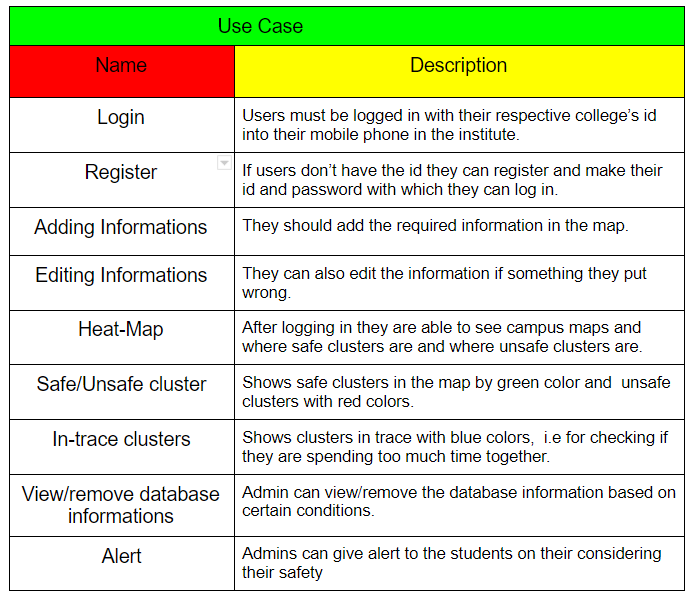
\includegraphics[width=9cm, height=8cm]{use cases.png}
\\ \\ \\ \\
Below is the Use case Table Use case diagram
\\ \\ \\
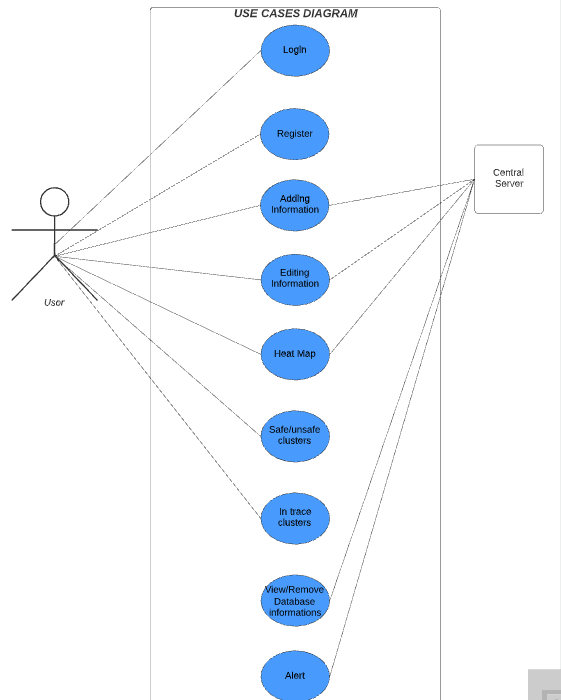
\includegraphics[width=9cm, height=8cm]{diagram.png}
\\


\section{Conclusion}
So basically the software system i proposed is that firstly our college is divided into 7 to 8 parts and each part will have 5 to robots and drons and each will do their respective work. Each student will have to keep his phone and it should be connected to the internet otherwise they will get an alert. This app will show them map on which every group is characterized as safe or unsafe and they or shown with different colors in the map. The main use of the app that it will give alert when you are unsafe or when you are near to unsafe group or when you are not wearing masks or when you spent a high amount of time within a group. Thus, this system will help in crowd detection and counting, mask detection basically it will help in monitoring and hence it will help in reducing the number of increasing cases in the campus.

{\small
\bibliographystyle{ieee}
\bibliography{egbib}
\begin{document}

\href{https://www.researchgate.net/publication/335490585_MRCNet_Crowd_Counting_and_Density_Map_Estimation_in_Aerial_and_Ground_Imagery}{Link1}.
\\
\href{https://paperswithcode.com/paper/mrcnet-crowd-counting-and-density-map/review/}{Link2}.
\\
\href{https://www.pyimagesearch.com/2020/05/04/covid-19-face-mask-detector-with-opencv-keras-tensorflow-and-deep-learning/}{Link3}.
\\
\href{https://ieeexplore.ieee.org/document/9342585}{Link4}.
\\
\href{https://global.canon/en/technology/count2019.html#:~:text=Canon's%20crowd%20counting%20technology%20uses,Canon's%20research%20into%20deep%20learning.}{Link5}.
\end{document}
}
\end{document}
\end{document}
